\documentclass[9pt]{beamer}
\usetheme{Berkeley}
\usepackage{multicol}
\usepackage{graphicx}
\linespread{1.35}
\usepackage{amsmath}
\usepackage{color}
\usepackage{xcolor}
\usepackage{tikz}
\usetikzlibrary{arrows,automata}


\begin{document}

\begin{frame}

\begin{flushright}
\texttt{Finite State Machine} \hspace*{0.10cm}\textbf{$|$} \textbf{137}\hspace*{0.5cm}
\end{flushright}

\section*{Sequence Detector}

\vspace*{1cm}
After doing this state assignment, the state table becomes
\begin{center}
\section{picture}
\includegraphics[width=8cm,height=3cm]{137-3.png}
\end{center}
\end{frame}

\begin{frame}
From this state assignment table, the digital function can easily be derived as follows.
\begin{center}
\section{picture}
\includegraphics[width=9cm,height=3cm]{137-1.png}
\end{center}

\begin{center}
$Y_1 = X'y'_1y_2 + Xy_1y_2 + X'y_1y'_2$\\
$Y_2 = y'_1y_2 + y'_1X + y_1y_2'$\\
$z = X'y_1y'_2$\\
\end{center}
\end{frame}

\begin{frame}
\hspace*{0.2cm} $Y_1$ and $Y_2$ are the next states, which are the memory elements. These will be feedbacked to the input
as states $y_1$ and $y_2$ with some delay by D flip flop. The circuit diagram is shown in Fig. 4.6.

\pause
\begin{center}
\section{picture}
\includegraphics[width=9cm,height=5cm]{137-2.png}
\end{center}
\end{frame}

\begin{frame}
\section*{Binary Counter}
\begin{flushleft}
    \textbf{138}\hspace*{0.1cm} \textbf{$|$} \hspace*{0.1cm} \texttt{Introduction to Automata Theory, Formal Languages and Computation}
  \end{flushleft}

  \vspace*{0.5cm}
  \textbf{4.2 Binary Counter}\\

  \vspace*{0.2cm}
  The binary counter counts in binary.\\

   \vspace*{0.2cm}
  \fcolorbox{red}{blue}{\textbf{Example 4.3}}\hspace*{0.1cm} \texttt{Design a Modulo 3 binary counter.}\\

  \textbf{Solution:} A Modulo 3 binary counter can count up to 3. The binary representation of 3 is 11. It can count
00, 01, 10, and 11. There will be an external input x, which will act as a control variable and determine
when the count should proceed. After counting 3, if it has to proceed, then it will come back to 00 again.
The state diagram for a Mod 3 binary counter is given in Fig. 4.7.\\
\end{frame}

\begin{frame}
\begin{center}
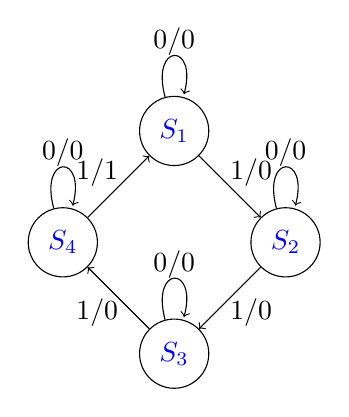
\begin{tikzpicture}[node distance = 2cm,auto,inner sep=0pt]
\node[state,text=blue,draw=black] (A) {$S_1$};
\node[state,text=blue,draw=black] (B) [below right of = A]  {$S_2$};
\node[state,text=blue,draw=black] (C) [below left of = B]  {$S_3$};
\node[state,text=blue,draw=black] (D) [above left of = C]  {$S_4$};


\path (A) edge [->] node {$1/0$} (B);
\path (B) edge [->] node {$1/0$} (C);
\path (C) edge [->] node {$1/0$} (D);
\path (D) edge [->] node {$1/1$} (A);
\path (A) edge [->,loop above] node {$0/0$} (A);
\path (B) edge [->,loop above] node {$0/0$} (B);
\path (C) edge [->,loop above] node {$0/0$} (C);
\path (D) edge [->,loop above] node {$0/0$} (D);

\end{tikzpicture}
\end{center}
\begin{center}
\textbf{Fig. 4.7} \hspace*{0.3cm} \texttt{State Diagram of a Mod 3 Binary Counter}
\end{center}
\end{frame}

\begin{frame}
The state table for Mod 3 binary counter is

\vspace*{0.3cm}
\begin{center}
\begin{tabular}{ccc}
 \hline

 \hline

 \hline

 \hline
 & \multicolumn{2}{c}{$Next State, O/P$}\\
 \cline{2-3}
 $Present State$ &  $X=0$ & $X=1$\\
\hline
 $S_1$    &    $S_1,0$    &   $S_2,0$  \\
 $S_2$    &    $S_2,0$    &   $S_3,0$  \\
 $S_3$    &    $S_3,0$    &   $S_4,0$  \\
 $S_4$    &    $S_4,0$    &   $S_1,1$  \\

 \hline

 \hline

 \hline

 \hline
\end{tabular}
\end{center}

\vspace*{0.3cm}
 \hspace*{0.2cm} There are four states in the machine. Two bits are sufficient to assign four states into the binary
number.\\
\end{frame}

\begin{frame}
 \hspace*{0.2cm} Let us assign $S_1$ to $00$, $S_2$ to $01$, $S_3$ to $10$, and $S_4$ to $11$.\\
 \hspace*{0.2cm} After doing this state assignment, the state table becomes\\

\vspace*{0.3cm}
\pause
\begin{center}
\section{picture}
\includegraphics[width=8cm,height=3cm]{138.png}
\end{center}
\end{frame}

\begin{frame}
\begin{flushright}
\texttt{Finite State Machine} \hspace*{0.10cm}\textbf{$|$} \textbf{139}\hspace*{0.5cm}
\end{flushright}

\section*{Binary Counter}

\vspace*{0.5cm}
\textbf{4.2.1 Designing Using Flip Flop (T Flip Flop and $SR$ Flip Flop)}\\

\vspace*{0.2cm}
The excitation table for T fl ip fl op is given in the following:

\pause
\begin{center}
\begin{tabular}{ccc}
 \hline

 \hline

 \hline

 \hline
 $Circuit From$ &  $Changed To$ & $T$\\
\hline
 $0$    &    $0$    &   $0$  \\
 $0$    &    $1$    &   $1$  \\
 $1$    &    $0$    &   $1$  \\
 $1$    &    $1$    &   $0$  \\
 \hline

 \hline

 \hline

 \hline
\end{tabular}
\end{center}
\end{frame}

\begin{frame}
\hspace*{0.2cm} In state assignment, 00 is changed to 00 for input 0. Here, $y_1$ is changed from 0 to 0, and so T1 will be 0.
$y_2$ is changed from 0 to 1, and so $T_1$ will be 0. 00 is changed to 01 for input 1. Here, $y_1$ is changed from 0
to 1, and so T1 will be 1. $y_2$ is changed from 0 to 0, and so $T_1$ will be 0. By this process, the excitation table
of the counter using T fl ip fl op is given in the following table.\\

\vspace*{0.1cm}
\pause
\begin{center}
\begin{tabular}{ccc}
 \hline

 \hline

 \hline

 \hline
$Present State$ & \multicolumn{2}{c}{$T_2T_1$}\\
 \cline{2-3}
 $(Y_2Y_1)$ &  $X=0$ & $X=1$\\
\hline
 $00$    &    $00$    &   $01$  \\
 $01$    &    $00$    &   $11$  \\
 $10$    &    $00$    &   $01$  \\
 $11$    &    $00$    &   $11$  \\

 \hline

 \hline

 \hline

 \hline
\end{tabular}
\end{center}

\pause
\begin{center}
  $T_1 = X$\\
  $T_2 = Xy_1$\\
  $z = Xy_1y_2$\\
\end{center}
\end{frame}

\begin{frame}
The circuit diagram for this is presented in Fig. 4.8.
\begin{center}
\section{picture}
\includegraphics[width=7cm,height=2cm]{139.png}
\end{center}

\pause
The excitation table for $SR$ flip flop is denoted in the following table.\\
\begin{center}
\begin{tabular}{cccc}
 \hline

 \hline

 \hline

 \hline
 $Circuit From$ &  $Changed To$ & $S$   &  $R$\\
\hline
 $0$    &    $0$    &   $0$   &  $-$\\
 $0$    &    $1$    &   $1$   &  $0$\\
 $1$    &    $0$    &   $1$   &  $1$\\
 $1$    &    $1$    &   $-$   &  $0$\\
 \hline

 \hline

 \hline

 \hline
\end{tabular}
\end{center}
\end{frame}

\begin{frame}
\section*{Binary Counter}
\begin{flushleft}
    \textbf{140}\hspace*{0.1cm} \textbf{$|$} \hspace*{0.1cm} \texttt{Introduction to Automata Theory, Formal Languages and Computation}
  \end{flushleft}

  \vspace*{2cm}
 \hspace*{0.2cm} In state assignment, $00$ is changed to $00$ for input $0$. Here, $y_1$ is changed from $0$ to $0$, and so $R_1$ will
be don’t care and $S_1$ will be $0$. $y_2$ is changed from $0$ to $0$, and so $R_2$ will be don’t care and $S_2$ will be $0$.\\
In the state assignment table, $00$ is changed to $01$ for input $1$. Here, $y_1$ is changed from $0$ to $1$, and so $R_1$
will be $0$ and $S_1$ will be $1$. $y_2$ is changed from $0$ to $0$, and so $R_2$ will be don’t care and $S_2$ will be $0$. By this
process, the excitation table of the counter using $SR$ flip flop is given as follows.\\
\end{frame}

\begin{frame}
\begin{center}
\section{picture}
\includegraphics[width=7cm,height=4cm]{140-1.png}
\end{center}

The circuit diagram for this is presented in Fig. 4.9.
\end{frame}

\begin{frame}
\begin{center}
\section{picture}
\includegraphics[width=9cm,height=5cm]{140.png}
\end{center}

\fcolorbox{red}{blue}{\textbf{Example 4.4}}\hspace*{0.1cm} \texttt{Design a Modulo $8$ binary counter}\\

\textbf{Solution:} A Modulo $8$ binary counter can count up to $8$ from $000$ to $111$. There will be an external input x,
which will act as a control variable and determine when the count should proceed. After counting $8$, if it
has to proceed, then it will come back to $000$ again.
\end{frame}
\end{document} 